% =====================================================================
%  Laboratorio de la Sesión 2: k-medias con el conjunto Iris
%  Se incluye desde Sesion2-KMedias.tex con % =====================================================================
%  Laboratorio de la Sesión 2: k-medias con el conjunto Iris
%  Se incluye desde Sesion2-KMedias.tex con % =====================================================================
%  Laboratorio de la Sesión 2: k-medias con el conjunto Iris
%  Se incluye desde Sesion2-KMedias.tex con % =====================================================================
%  Laboratorio de la Sesión 2: k-medias con el conjunto Iris
%  Se incluye desde Sesion2-KMedias.tex con \input{Laboratorio}
% =====================================================================
\section{Laboratorio: k-medias con Iris}
% =====================================================================

\begin{frame}[fragile]{Paso 1: cargar y explorar los datos}
\begin{lstlisting}
import numpy as np, pandas as pd
from sklearn.datasets import load_iris

iris = load_iris(as_frame=True)
X = iris.data                  # 150 x 4, medidas en cm
especie = iris.target          # se guarda aparte: NO se usa para agrupar

print(X.describe().T[["mean", "std", "min", "max"]])
\end{lstlisting}
  \vspace{2pt}
  \centering
  \small
  \begin{tabular}{@{}lcccc@{}}
    \toprule
    \textbf{Variable (cm)} & \textbf{Media} & \textbf{Desv.\ est.} & \textbf{Mín.} & \textbf{Máx.}\\
    \midrule
    Largo del sépalo & 5.84 & 0.83 & 4.3 & 7.9 \\
    Ancho del sépalo & 3.06 & 0.44 & 2.0 & 4.4 \\
    Largo del pétalo & 3.76 & 1.77 & 1.0 & 6.9 \\
    Ancho del pétalo & 1.20 & 0.76 & 0.1 & 2.5 \\
    \bottomrule
  \end{tabular}\\[4pt]
  \raggedright
  {\small Las cuatro variables están en la misma unidad. Los pétalos tienen la mayor variación.}
\end{frame}

\begin{frame}[fragile]{Paso 2: elegir $k$}
\begin{lstlisting}
from sklearn.cluster import KMeans
from sklearn.metrics import silhouette_score

for k in range(2, 9):
    km = KMeans(n_clusters=k, n_init=10, random_state=0).fit(X)
    print(k, round(km.inertia_, 1), round(silhouette_score(X, km.labels_), 3))
\end{lstlisting}
  \centering
  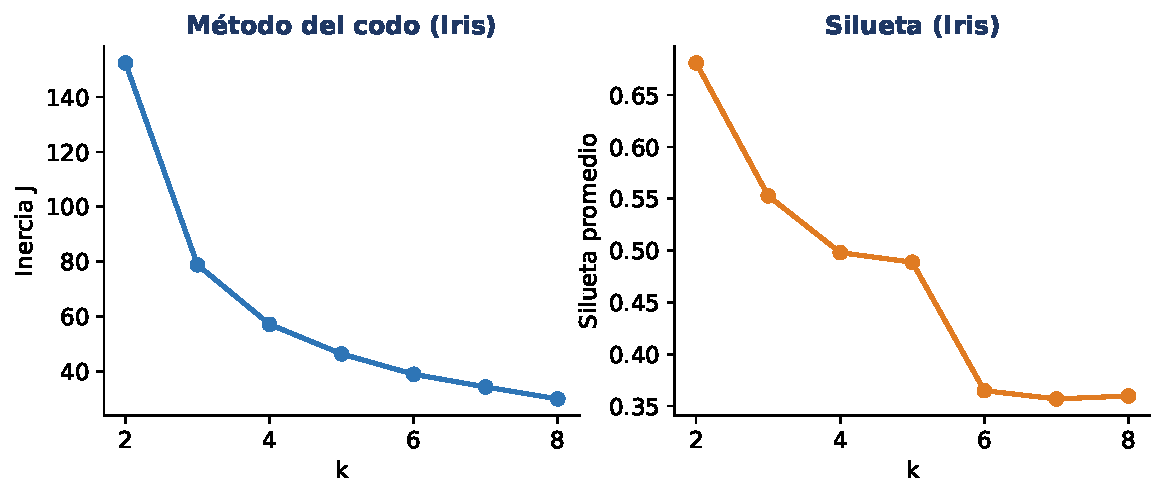
\includegraphics[width=0.62\textwidth]{iris_codo_silueta}\\
  \raggedright
  {\small El codo aparece entre $k=2$ y $k=3$. La silueta es máxima con $k=2$ (0.68) y baja a 0.55 con $k=3$.}
\end{frame}

\begin{frame}{Paso 2: ¿dos o tres grupos?}
  \begin{itemize}
    \item Los criterios numéricos sugieren $k=2$: una especie (setosa) está muy separada
          y las otras dos se traslapan.
    \item Con $k=3$ el codo todavía muestra una reducción importante de $J$ (de 152 a 79).
    \item Sabemos por el dominio que esperamos tres tipos de flor: elegimos $k=3$.
  \end{itemize}
  \vspace{6pt}
  \begin{alertblock}{Lección}
    La silueta mide qué tan separados quedan los grupos, no si corresponden a categorías reales.
    La elección de $k$ combina criterios numéricos y conocimiento del problema.
  \end{alertblock}
\end{frame}

\begin{frame}[fragile]{Paso 3: ajustar e interpretar los centros}
\begin{lstlisting}
km = KMeans(n_clusters=3, n_init=10, random_state=0).fit(X)
centros = pd.DataFrame(km.cluster_centers_, columns=X.columns)
print(centros.round(2)); print(np.bincount(km.labels_))
\end{lstlisting}
  \vspace{2pt}
  \centering
  \small
  \begin{tabular}{@{}lccccc@{}}
    \toprule
    \textbf{Grupo} & \textbf{Largo sépalo} & \textbf{Ancho sépalo} & \textbf{Largo pétalo} & \textbf{Ancho pétalo} & \textbf{Flores}\\
    \midrule
    A & 5.01 & 3.43 & 1.46 & 0.25 & 50 \\
    B & 5.90 & 2.75 & 4.39 & 1.43 & 62 \\
    C & 6.85 & 3.07 & 5.74 & 2.07 & 38 \\
    \bottomrule
  \end{tabular}\\[6pt]
  \raggedright
  \begin{itemize}
    \item Grupo A: pétalos pequeños y sépalos anchos.
    \item Grupos B y C: pétalos medianos y grandes, respectivamente.
  \end{itemize}
  {\small Los centros están en centímetros: se interpretan directamente como una flor ``típica'' de cada grupo.}
\end{frame}

\begin{frame}[fragile]{Paso 4: comparar con las especies}
\begin{lstlisting}
from sklearn.metrics import adjusted_rand_score
print(pd.crosstab(km.labels_, iris.target_names[especie]))
print(adjusted_rand_score(especie, km.labels_))   # 1 = coincidencia perfecta (S6)
\end{lstlisting}
  \begin{columns}[c]
    \column{0.58\textwidth}
    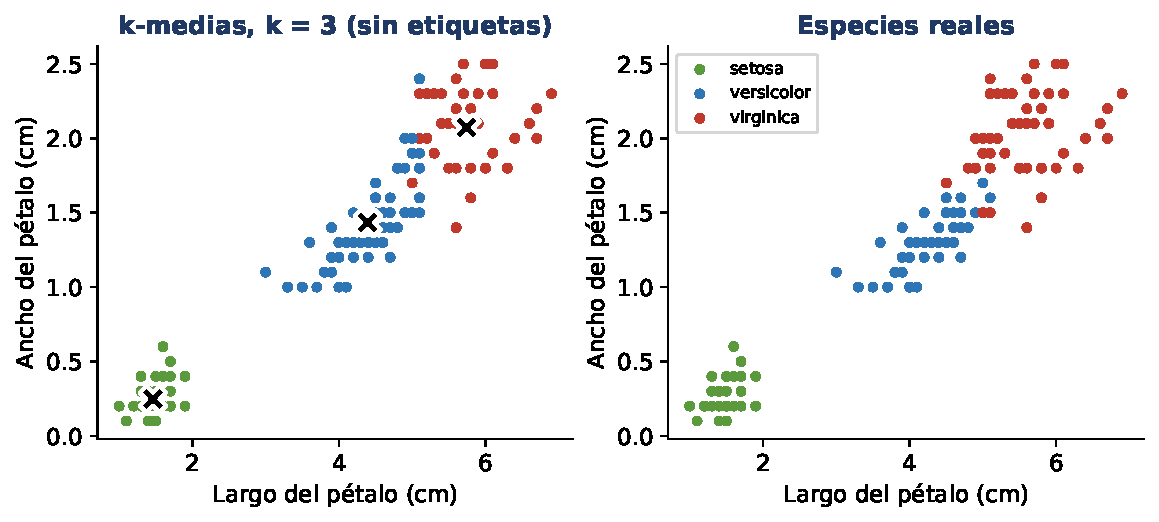
\includegraphics[width=\textwidth]{iris_resultado}
    \column{0.4\textwidth}
    \small
    \begin{tabular}{@{}lccc@{}}
      \toprule
      & \textbf{setosa} & \textbf{versic.} & \textbf{virgin.}\\
      \midrule
      A & 50 & 0 & 0 \\
      B & 0 & 48 & 14 \\
      C & 0 & 2 & 36 \\
      \bottomrule
    \end{tabular}\\[4pt]
    \begin{itemize}
      \item Setosa se recupera sin errores.
      \item 16 flores quedan en la frontera entre versicolor y virginica.
      \item Índice de Rand ajustado: 0.73.
    \end{itemize}
  \end{columns}
\end{frame}

\begin{frame}[fragile]{Paso 5: ¿conviene estandarizar?}
\begin{lstlisting}
from sklearn.pipeline import make_pipeline
from sklearn.preprocessing import StandardScaler

km_std = make_pipeline(StandardScaler(), KMeans(n_clusters=3, n_init=10, random_state=0))
etiquetas_std = km_std.fit_predict(X)
print(adjusted_rand_score(especie, etiquetas_std))
\end{lstlisting}
  \centering
  \small
  \begin{tabular}{@{}lcc@{}}
    \toprule
    \textbf{Datos ($k=3$)} & \textbf{Silueta} & \textbf{Rand ajustado}\\
    \midrule
    En centímetros & 0.55 & 0.73 \\
    Estandarizados & 0.46 & 0.62 \\
    \bottomrule
  \end{tabular}\\[6pt]
  \raggedright
  \begin{itemize}
    \item Aquí todas las variables tienen la misma unidad: estandarizar \alert{no es necesario}.
    \item Al estandarizar, el ancho del sépalo pesa lo mismo que los pétalos, que son más
          informativos, y el resultado empeora.
    \item Estandarizar es la regla cuando las unidades difieren (Sesión 1); no es automático.
  \end{itemize}
\end{frame}

\begin{frame}{Conclusiones del laboratorio}
  \begin{itemize}
    \item Sin usar la especie, k-medias descubre la estructura principal de Iris:
          un grupo bien separado y dos que se traslapan.
    \item Los criterios numéricos (silueta) sugieren $k=2$; el conocimiento del dominio lleva a $k=3$.
    \item Los centros, en las unidades originales, permiten describir cada grupo.
    \item Las decisiones de preprocesamiento cambian el resultado: deben justificarse.
    \item Las flores mal asignadas están en la frontera entre especies parecidas:
          k-medias asigna cada punto a un solo grupo, sin expresar incertidumbre
          (lo resolverán las mezclas gaussianas, Sesión 4).
  \end{itemize}
\end{frame}

% =====================================================================
\section{Laboratorio: k-medias con Iris}
% =====================================================================

\begin{frame}[fragile]{Paso 1: cargar y explorar los datos}
\begin{lstlisting}
import numpy as np, pandas as pd
from sklearn.datasets import load_iris

iris = load_iris(as_frame=True)
X = iris.data                  # 150 x 4, medidas en cm
especie = iris.target          # se guarda aparte: NO se usa para agrupar

print(X.describe().T[["mean", "std", "min", "max"]])
\end{lstlisting}
  \vspace{2pt}
  \centering
  \small
  \begin{tabular}{@{}lcccc@{}}
    \toprule
    \textbf{Variable (cm)} & \textbf{Media} & \textbf{Desv.\ est.} & \textbf{Mín.} & \textbf{Máx.}\\
    \midrule
    Largo del sépalo & 5.84 & 0.83 & 4.3 & 7.9 \\
    Ancho del sépalo & 3.06 & 0.44 & 2.0 & 4.4 \\
    Largo del pétalo & 3.76 & 1.77 & 1.0 & 6.9 \\
    Ancho del pétalo & 1.20 & 0.76 & 0.1 & 2.5 \\
    \bottomrule
  \end{tabular}\\[4pt]
  \raggedright
  {\small Las cuatro variables están en la misma unidad. Los pétalos tienen la mayor variación.}
\end{frame}

\begin{frame}[fragile]{Paso 2: elegir $k$}
\begin{lstlisting}
from sklearn.cluster import KMeans
from sklearn.metrics import silhouette_score

for k in range(2, 9):
    km = KMeans(n_clusters=k, n_init=10, random_state=0).fit(X)
    print(k, round(km.inertia_, 1), round(silhouette_score(X, km.labels_), 3))
\end{lstlisting}
  \centering
  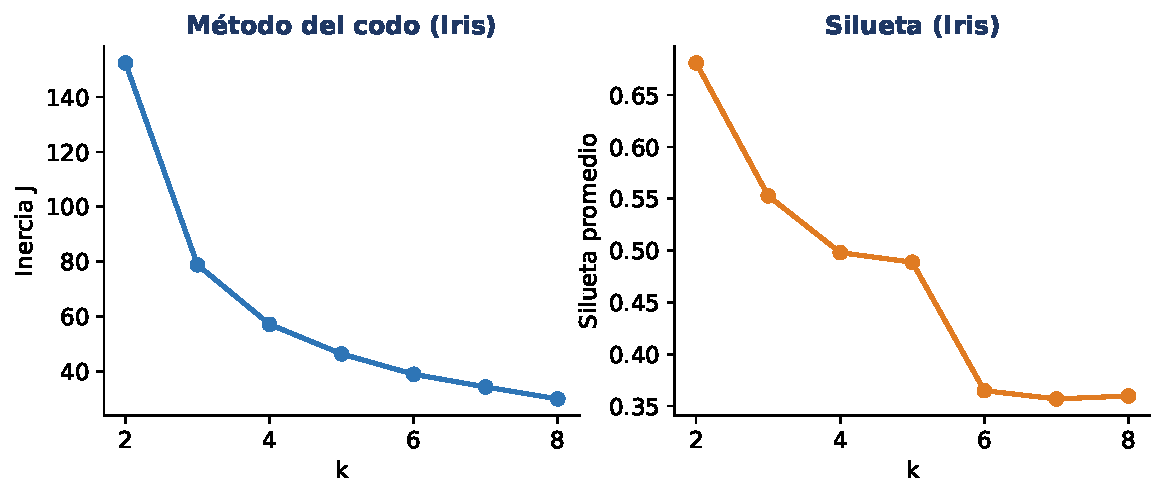
\includegraphics[width=0.62\textwidth]{iris_codo_silueta}\\
  \raggedright
  {\small El codo aparece entre $k=2$ y $k=3$. La silueta es máxima con $k=2$ (0.68) y baja a 0.55 con $k=3$.}
\end{frame}

\begin{frame}{Paso 2: ¿dos o tres grupos?}
  \begin{itemize}
    \item Los criterios numéricos sugieren $k=2$: una especie (setosa) está muy separada
          y las otras dos se traslapan.
    \item Con $k=3$ el codo todavía muestra una reducción importante de $J$ (de 152 a 79).
    \item Sabemos por el dominio que esperamos tres tipos de flor: elegimos $k=3$.
  \end{itemize}
  \vspace{6pt}
  \begin{alertblock}{Lección}
    La silueta mide qué tan separados quedan los grupos, no si corresponden a categorías reales.
    La elección de $k$ combina criterios numéricos y conocimiento del problema.
  \end{alertblock}
\end{frame}

\begin{frame}[fragile]{Paso 3: ajustar e interpretar los centros}
\begin{lstlisting}
km = KMeans(n_clusters=3, n_init=10, random_state=0).fit(X)
centros = pd.DataFrame(km.cluster_centers_, columns=X.columns)
print(centros.round(2)); print(np.bincount(km.labels_))
\end{lstlisting}
  \vspace{2pt}
  \centering
  \small
  \begin{tabular}{@{}lccccc@{}}
    \toprule
    \textbf{Grupo} & \textbf{Largo sépalo} & \textbf{Ancho sépalo} & \textbf{Largo pétalo} & \textbf{Ancho pétalo} & \textbf{Flores}\\
    \midrule
    A & 5.01 & 3.43 & 1.46 & 0.25 & 50 \\
    B & 5.90 & 2.75 & 4.39 & 1.43 & 62 \\
    C & 6.85 & 3.07 & 5.74 & 2.07 & 38 \\
    \bottomrule
  \end{tabular}\\[6pt]
  \raggedright
  \begin{itemize}
    \item Grupo A: pétalos pequeños y sépalos anchos.
    \item Grupos B y C: pétalos medianos y grandes, respectivamente.
  \end{itemize}
  {\small Los centros están en centímetros: se interpretan directamente como una flor ``típica'' de cada grupo.}
\end{frame}

\begin{frame}[fragile]{Paso 4: comparar con las especies}
\begin{lstlisting}
from sklearn.metrics import adjusted_rand_score
print(pd.crosstab(km.labels_, iris.target_names[especie]))
print(adjusted_rand_score(especie, km.labels_))   # 1 = coincidencia perfecta (S6)
\end{lstlisting}
  \begin{columns}[c]
    \column{0.58\textwidth}
    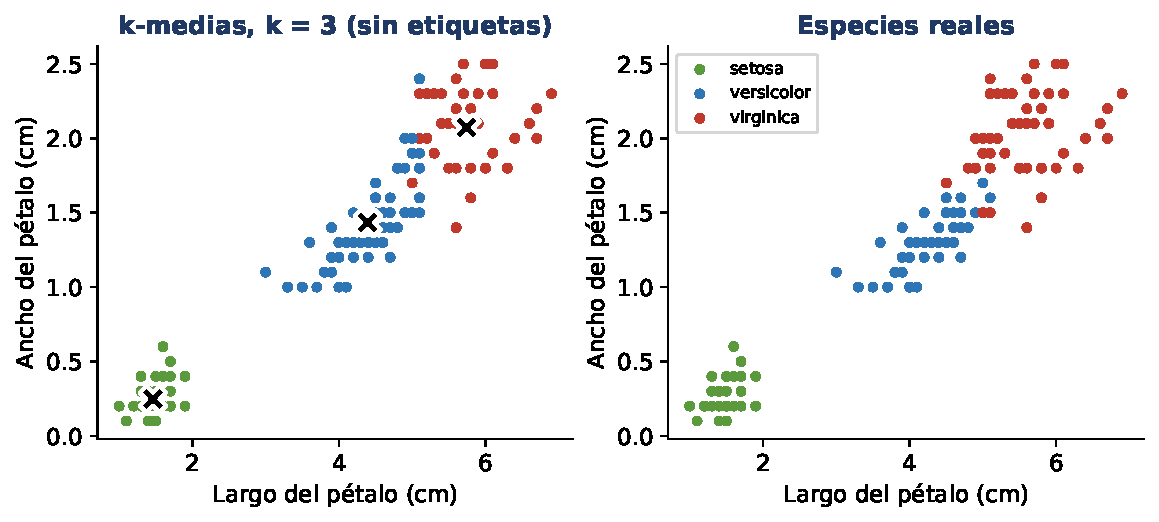
\includegraphics[width=\textwidth]{iris_resultado}
    \column{0.4\textwidth}
    \small
    \begin{tabular}{@{}lccc@{}}
      \toprule
      & \textbf{setosa} & \textbf{versic.} & \textbf{virgin.}\\
      \midrule
      A & 50 & 0 & 0 \\
      B & 0 & 48 & 14 \\
      C & 0 & 2 & 36 \\
      \bottomrule
    \end{tabular}\\[4pt]
    \begin{itemize}
      \item Setosa se recupera sin errores.
      \item 16 flores quedan en la frontera entre versicolor y virginica.
      \item Índice de Rand ajustado: 0.73.
    \end{itemize}
  \end{columns}
\end{frame}

\begin{frame}[fragile]{Paso 5: ¿conviene estandarizar?}
\begin{lstlisting}
from sklearn.pipeline import make_pipeline
from sklearn.preprocessing import StandardScaler

km_std = make_pipeline(StandardScaler(), KMeans(n_clusters=3, n_init=10, random_state=0))
etiquetas_std = km_std.fit_predict(X)
print(adjusted_rand_score(especie, etiquetas_std))
\end{lstlisting}
  \centering
  \small
  \begin{tabular}{@{}lcc@{}}
    \toprule
    \textbf{Datos ($k=3$)} & \textbf{Silueta} & \textbf{Rand ajustado}\\
    \midrule
    En centímetros & 0.55 & 0.73 \\
    Estandarizados & 0.46 & 0.62 \\
    \bottomrule
  \end{tabular}\\[6pt]
  \raggedright
  \begin{itemize}
    \item Aquí todas las variables tienen la misma unidad: estandarizar \alert{no es necesario}.
    \item Al estandarizar, el ancho del sépalo pesa lo mismo que los pétalos, que son más
          informativos, y el resultado empeora.
    \item Estandarizar es la regla cuando las unidades difieren (Sesión 1); no es automático.
  \end{itemize}
\end{frame}

\begin{frame}{Conclusiones del laboratorio}
  \begin{itemize}
    \item Sin usar la especie, k-medias descubre la estructura principal de Iris:
          un grupo bien separado y dos que se traslapan.
    \item Los criterios numéricos (silueta) sugieren $k=2$; el conocimiento del dominio lleva a $k=3$.
    \item Los centros, en las unidades originales, permiten describir cada grupo.
    \item Las decisiones de preprocesamiento cambian el resultado: deben justificarse.
    \item Las flores mal asignadas están en la frontera entre especies parecidas:
          k-medias asigna cada punto a un solo grupo, sin expresar incertidumbre
          (lo resolverán las mezclas gaussianas, Sesión 4).
  \end{itemize}
\end{frame}

% =====================================================================
\section{Laboratorio: k-medias con Iris}
% =====================================================================

\begin{frame}[fragile]{Paso 1: cargar y explorar los datos}
\begin{lstlisting}
import numpy as np, pandas as pd
from sklearn.datasets import load_iris

iris = load_iris(as_frame=True)
X = iris.data                  # 150 x 4, medidas en cm
especie = iris.target          # se guarda aparte: NO se usa para agrupar

print(X.describe().T[["mean", "std", "min", "max"]])
\end{lstlisting}
  \vspace{2pt}
  \centering
  \small
  \begin{tabular}{@{}lcccc@{}}
    \toprule
    \textbf{Variable (cm)} & \textbf{Media} & \textbf{Desv.\ est.} & \textbf{Mín.} & \textbf{Máx.}\\
    \midrule
    Largo del sépalo & 5.84 & 0.83 & 4.3 & 7.9 \\
    Ancho del sépalo & 3.06 & 0.44 & 2.0 & 4.4 \\
    Largo del pétalo & 3.76 & 1.77 & 1.0 & 6.9 \\
    Ancho del pétalo & 1.20 & 0.76 & 0.1 & 2.5 \\
    \bottomrule
  \end{tabular}\\[4pt]
  \raggedright
  {\small Las cuatro variables están en la misma unidad. Los pétalos tienen la mayor variación.}
\end{frame}

\begin{frame}[fragile]{Paso 2: elegir $k$}
\begin{lstlisting}
from sklearn.cluster import KMeans
from sklearn.metrics import silhouette_score

for k in range(2, 9):
    km = KMeans(n_clusters=k, n_init=10, random_state=0).fit(X)
    print(k, round(km.inertia_, 1), round(silhouette_score(X, km.labels_), 3))
\end{lstlisting}
  \centering
  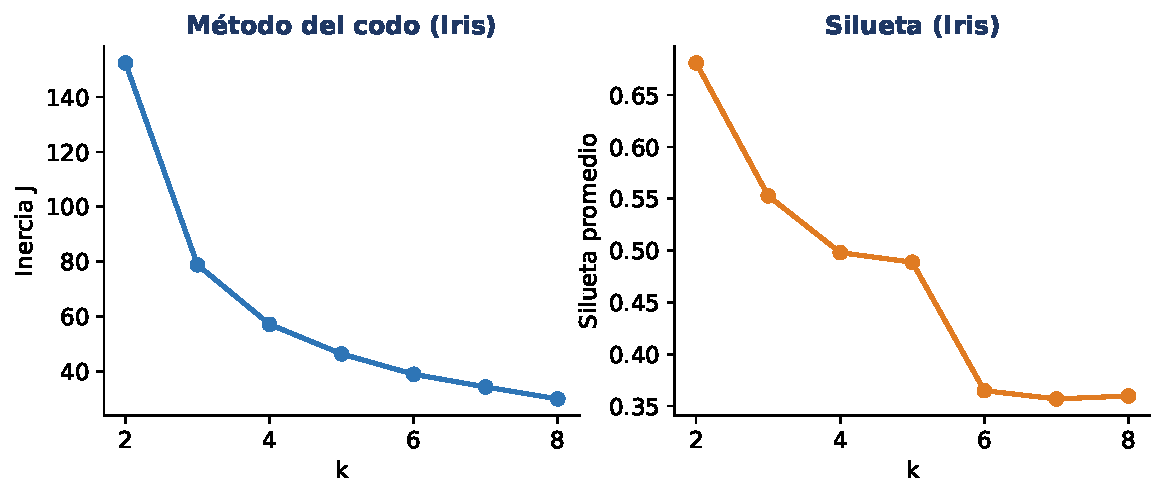
\includegraphics[width=0.62\textwidth]{iris_codo_silueta}\\
  \raggedright
  {\small El codo aparece entre $k=2$ y $k=3$. La silueta es máxima con $k=2$ (0.68) y baja a 0.55 con $k=3$.}
\end{frame}

\begin{frame}{Paso 2: ¿dos o tres grupos?}
  \begin{itemize}
    \item Los criterios numéricos sugieren $k=2$: una especie (setosa) está muy separada
          y las otras dos se traslapan.
    \item Con $k=3$ el codo todavía muestra una reducción importante de $J$ (de 152 a 79).
    \item Sabemos por el dominio que esperamos tres tipos de flor: elegimos $k=3$.
  \end{itemize}
  \vspace{6pt}
  \begin{alertblock}{Lección}
    La silueta mide qué tan separados quedan los grupos, no si corresponden a categorías reales.
    La elección de $k$ combina criterios numéricos y conocimiento del problema.
  \end{alertblock}
\end{frame}

\begin{frame}[fragile]{Paso 3: ajustar e interpretar los centros}
\begin{lstlisting}
km = KMeans(n_clusters=3, n_init=10, random_state=0).fit(X)
centros = pd.DataFrame(km.cluster_centers_, columns=X.columns)
print(centros.round(2)); print(np.bincount(km.labels_))
\end{lstlisting}
  \vspace{2pt}
  \centering
  \small
  \begin{tabular}{@{}lccccc@{}}
    \toprule
    \textbf{Grupo} & \textbf{Largo sépalo} & \textbf{Ancho sépalo} & \textbf{Largo pétalo} & \textbf{Ancho pétalo} & \textbf{Flores}\\
    \midrule
    A & 5.01 & 3.43 & 1.46 & 0.25 & 50 \\
    B & 5.90 & 2.75 & 4.39 & 1.43 & 62 \\
    C & 6.85 & 3.07 & 5.74 & 2.07 & 38 \\
    \bottomrule
  \end{tabular}\\[6pt]
  \raggedright
  \begin{itemize}
    \item Grupo A: pétalos pequeños y sépalos anchos.
    \item Grupos B y C: pétalos medianos y grandes, respectivamente.
  \end{itemize}
  {\small Los centros están en centímetros: se interpretan directamente como una flor ``típica'' de cada grupo.}
\end{frame}

\begin{frame}[fragile]{Paso 4: comparar con las especies}
\begin{lstlisting}
from sklearn.metrics import adjusted_rand_score
print(pd.crosstab(km.labels_, iris.target_names[especie]))
print(adjusted_rand_score(especie, km.labels_))   # 1 = coincidencia perfecta (S6)
\end{lstlisting}
  \begin{columns}[c]
    \column{0.58\textwidth}
    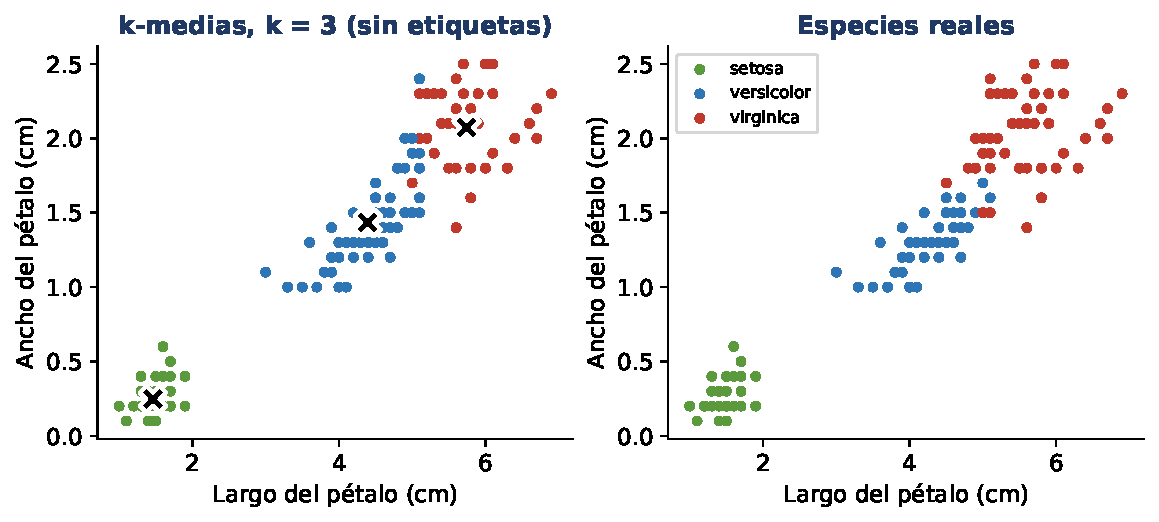
\includegraphics[width=\textwidth]{iris_resultado}
    \column{0.4\textwidth}
    \small
    \begin{tabular}{@{}lccc@{}}
      \toprule
      & \textbf{setosa} & \textbf{versic.} & \textbf{virgin.}\\
      \midrule
      A & 50 & 0 & 0 \\
      B & 0 & 48 & 14 \\
      C & 0 & 2 & 36 \\
      \bottomrule
    \end{tabular}\\[4pt]
    \begin{itemize}
      \item Setosa se recupera sin errores.
      \item 16 flores quedan en la frontera entre versicolor y virginica.
      \item Índice de Rand ajustado: 0.73.
    \end{itemize}
  \end{columns}
\end{frame}

\begin{frame}[fragile]{Paso 5: ¿conviene estandarizar?}
\begin{lstlisting}
from sklearn.pipeline import make_pipeline
from sklearn.preprocessing import StandardScaler

km_std = make_pipeline(StandardScaler(), KMeans(n_clusters=3, n_init=10, random_state=0))
etiquetas_std = km_std.fit_predict(X)
print(adjusted_rand_score(especie, etiquetas_std))
\end{lstlisting}
  \centering
  \small
  \begin{tabular}{@{}lcc@{}}
    \toprule
    \textbf{Datos ($k=3$)} & \textbf{Silueta} & \textbf{Rand ajustado}\\
    \midrule
    En centímetros & 0.55 & 0.73 \\
    Estandarizados & 0.46 & 0.62 \\
    \bottomrule
  \end{tabular}\\[6pt]
  \raggedright
  \begin{itemize}
    \item Aquí todas las variables tienen la misma unidad: estandarizar \alert{no es necesario}.
    \item Al estandarizar, el ancho del sépalo pesa lo mismo que los pétalos, que son más
          informativos, y el resultado empeora.
    \item Estandarizar es la regla cuando las unidades difieren (Sesión 1); no es automático.
  \end{itemize}
\end{frame}

\begin{frame}{Conclusiones del laboratorio}
  \begin{itemize}
    \item Sin usar la especie, k-medias descubre la estructura principal de Iris:
          un grupo bien separado y dos que se traslapan.
    \item Los criterios numéricos (silueta) sugieren $k=2$; el conocimiento del dominio lleva a $k=3$.
    \item Los centros, en las unidades originales, permiten describir cada grupo.
    \item Las decisiones de preprocesamiento cambian el resultado: deben justificarse.
    \item Las flores mal asignadas están en la frontera entre especies parecidas:
          k-medias asigna cada punto a un solo grupo, sin expresar incertidumbre
          (lo resolverán las mezclas gaussianas, Sesión 4).
  \end{itemize}
\end{frame}

% =====================================================================
\section{Laboratorio: k-medias con Iris}
% =====================================================================

\begin{frame}[fragile]{Paso 1: cargar y explorar los datos}
\begin{lstlisting}
import numpy as np, pandas as pd
from sklearn.datasets import load_iris

iris = load_iris(as_frame=True)
X = iris.data                  # 150 x 4, medidas en cm
especie = iris.target          # se guarda aparte: NO se usa para agrupar

print(X.describe().T[["mean", "std", "min", "max"]])
\end{lstlisting}
  \vspace{2pt}
  \centering
  \small
  \begin{tabular}{@{}lcccc@{}}
    \toprule
    \textbf{Variable (cm)} & \textbf{Media} & \textbf{Desv.\ est.} & \textbf{Mín.} & \textbf{Máx.}\\
    \midrule
    Largo del sépalo & 5.84 & 0.83 & 4.3 & 7.9 \\
    Ancho del sépalo & 3.06 & 0.44 & 2.0 & 4.4 \\
    Largo del pétalo & 3.76 & 1.77 & 1.0 & 6.9 \\
    Ancho del pétalo & 1.20 & 0.76 & 0.1 & 2.5 \\
    \bottomrule
  \end{tabular}\\[4pt]
  \raggedright
  {\small Las cuatro variables están en la misma unidad. Los pétalos tienen la mayor variación.}
\end{frame}

\begin{frame}[fragile]{Paso 2: elegir $k$}
\begin{lstlisting}
from sklearn.cluster import KMeans
from sklearn.metrics import silhouette_score

for k in range(2, 9):
    km = KMeans(n_clusters=k, n_init=10, random_state=0).fit(X)
    print(k, round(km.inertia_, 1), round(silhouette_score(X, km.labels_), 3))
\end{lstlisting}
  \centering
  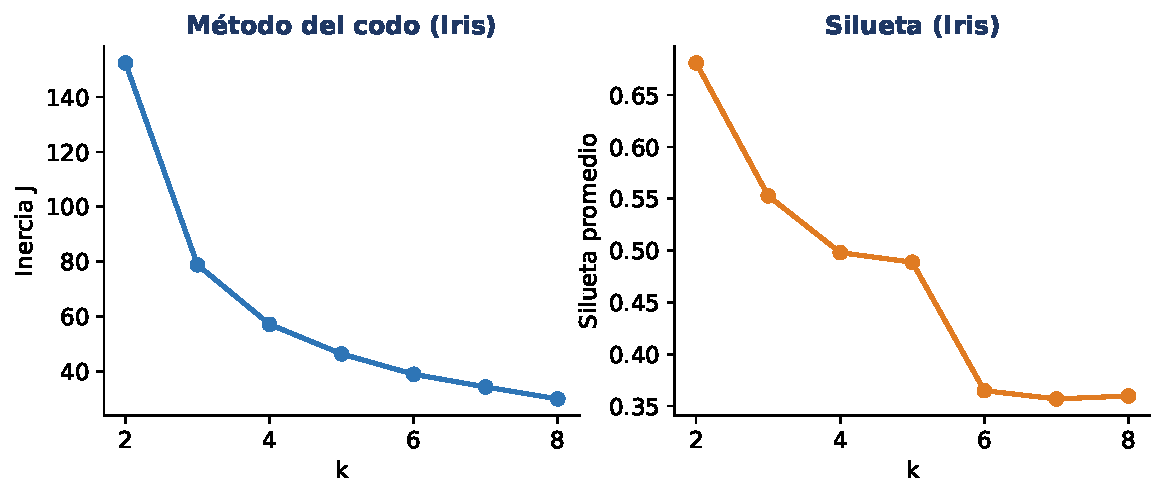
\includegraphics[width=0.62\textwidth]{iris_codo_silueta}\\
  \raggedright
  {\small El codo aparece entre $k=2$ y $k=3$. La silueta es máxima con $k=2$ (0.68) y baja a 0.55 con $k=3$.}
\end{frame}

\begin{frame}{Paso 2: ¿dos o tres grupos?}
  \begin{itemize}
    \item Los criterios numéricos sugieren $k=2$: una especie (setosa) está muy separada
          y las otras dos se traslapan.
    \item Con $k=3$ el codo todavía muestra una reducción importante de $J$ (de 152 a 79).
    \item Sabemos por el dominio que esperamos tres tipos de flor: elegimos $k=3$.
  \end{itemize}
  \vspace{6pt}
  \begin{alertblock}{Lección}
    La silueta mide qué tan separados quedan los grupos, no si corresponden a categorías reales.
    La elección de $k$ combina criterios numéricos y conocimiento del problema.
  \end{alertblock}
\end{frame}

\begin{frame}[fragile]{Paso 3: ajustar e interpretar los centros}
\begin{lstlisting}
km = KMeans(n_clusters=3, n_init=10, random_state=0).fit(X)
centros = pd.DataFrame(km.cluster_centers_, columns=X.columns)
print(centros.round(2)); print(np.bincount(km.labels_))
\end{lstlisting}
  \vspace{2pt}
  \centering
  \small
  \begin{tabular}{@{}lccccc@{}}
    \toprule
    \textbf{Grupo} & \textbf{Largo sépalo} & \textbf{Ancho sépalo} & \textbf{Largo pétalo} & \textbf{Ancho pétalo} & \textbf{Flores}\\
    \midrule
    A & 5.01 & 3.43 & 1.46 & 0.25 & 50 \\
    B & 5.90 & 2.75 & 4.39 & 1.43 & 62 \\
    C & 6.85 & 3.07 & 5.74 & 2.07 & 38 \\
    \bottomrule
  \end{tabular}\\[6pt]
  \raggedright
  \begin{itemize}
    \item Grupo A: pétalos pequeños y sépalos anchos.
    \item Grupos B y C: pétalos medianos y grandes, respectivamente.
  \end{itemize}
  {\small Los centros están en centímetros: se interpretan directamente como una flor ``típica'' de cada grupo.}
\end{frame}

\begin{frame}[fragile]{Paso 4: comparar con las especies}
\begin{lstlisting}
from sklearn.metrics import adjusted_rand_score
print(pd.crosstab(km.labels_, iris.target_names[especie]))
print(adjusted_rand_score(especie, km.labels_))   # 1 = coincidencia perfecta (S6)
\end{lstlisting}
  \begin{columns}[c]
    \column{0.58\textwidth}
    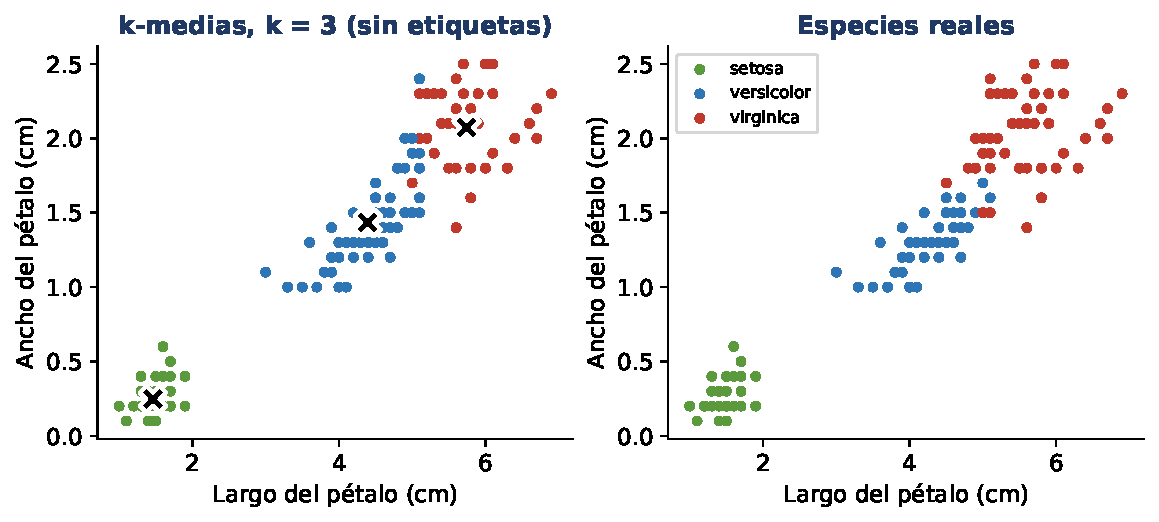
\includegraphics[width=\textwidth]{iris_resultado}
    \column{0.4\textwidth}
    \small
    \begin{tabular}{@{}lccc@{}}
      \toprule
      & \textbf{setosa} & \textbf{versic.} & \textbf{virgin.}\\
      \midrule
      A & 50 & 0 & 0 \\
      B & 0 & 48 & 14 \\
      C & 0 & 2 & 36 \\
      \bottomrule
    \end{tabular}\\[4pt]
    \begin{itemize}
      \item Setosa se recupera sin errores.
      \item 16 flores quedan en la frontera entre versicolor y virginica.
      \item Índice de Rand ajustado: 0.73.
    \end{itemize}
  \end{columns}
\end{frame}

\begin{frame}[fragile]{Paso 5: ¿conviene estandarizar?}
\begin{lstlisting}
from sklearn.pipeline import make_pipeline
from sklearn.preprocessing import StandardScaler

km_std = make_pipeline(StandardScaler(), KMeans(n_clusters=3, n_init=10, random_state=0))
etiquetas_std = km_std.fit_predict(X)
print(adjusted_rand_score(especie, etiquetas_std))
\end{lstlisting}
  \centering
  \small
  \begin{tabular}{@{}lcc@{}}
    \toprule
    \textbf{Datos ($k=3$)} & \textbf{Silueta} & \textbf{Rand ajustado}\\
    \midrule
    En centímetros & 0.55 & 0.73 \\
    Estandarizados & 0.46 & 0.62 \\
    \bottomrule
  \end{tabular}\\[6pt]
  \raggedright
  \begin{itemize}
    \item Aquí todas las variables tienen la misma unidad: estandarizar \alert{no es necesario}.
    \item Al estandarizar, el ancho del sépalo pesa lo mismo que los pétalos, que son más
          informativos, y el resultado empeora.
    \item Estandarizar es la regla cuando las unidades difieren (Sesión 1); no es automático.
  \end{itemize}
\end{frame}

\begin{frame}{Conclusiones del laboratorio}
  \begin{itemize}
    \item Sin usar la especie, k-medias descubre la estructura principal de Iris:
          un grupo bien separado y dos que se traslapan.
    \item Los criterios numéricos (silueta) sugieren $k=2$; el conocimiento del dominio lleva a $k=3$.
    \item Los centros, en las unidades originales, permiten describir cada grupo.
    \item Las decisiones de preprocesamiento cambian el resultado: deben justificarse.
    \item Las flores mal asignadas están en la frontera entre especies parecidas:
          k-medias asigna cada punto a un solo grupo, sin expresar incertidumbre
          (lo resolverán las mezclas gaussianas, Sesión 4).
  \end{itemize}
\end{frame}
